\subsection{Sound Processing}

%%ANGUS: for you to discuss how we achieved what's been specified in the intro - make subsubsections for like brief description of how we're using aubio, beat detection, clustering, etc...

%% fix the intro/background if you feel inaccurately describes the sound processing bits (doesn't need to be too detailed in the intro/background) - your time to shine is here and in section 4

Some sound processing modules were implemented sucessfully, while others were not perfect, requiring further refinement. The module that worked very effectivly was beat detection. Switching from tempo to onset detection worked very effectivly for song sections that did not contain a distinct beat, or sections with a changing tempo. Clustering of song sections also worked effectivly, providing a nice way to divide the song up into distinct and useable sections (see figure \ref{fig:cluster_output} and \ref{fig:clustering}). The component that was less affective was the classification (see figure \ref{fig:classification}. In hindsight, changes could have been made in the classification module to achieve more accurate and useful results (potential changes and improvements are covered in the discussion section.) \\
\\
\begin{figure}[H]
      \centering
      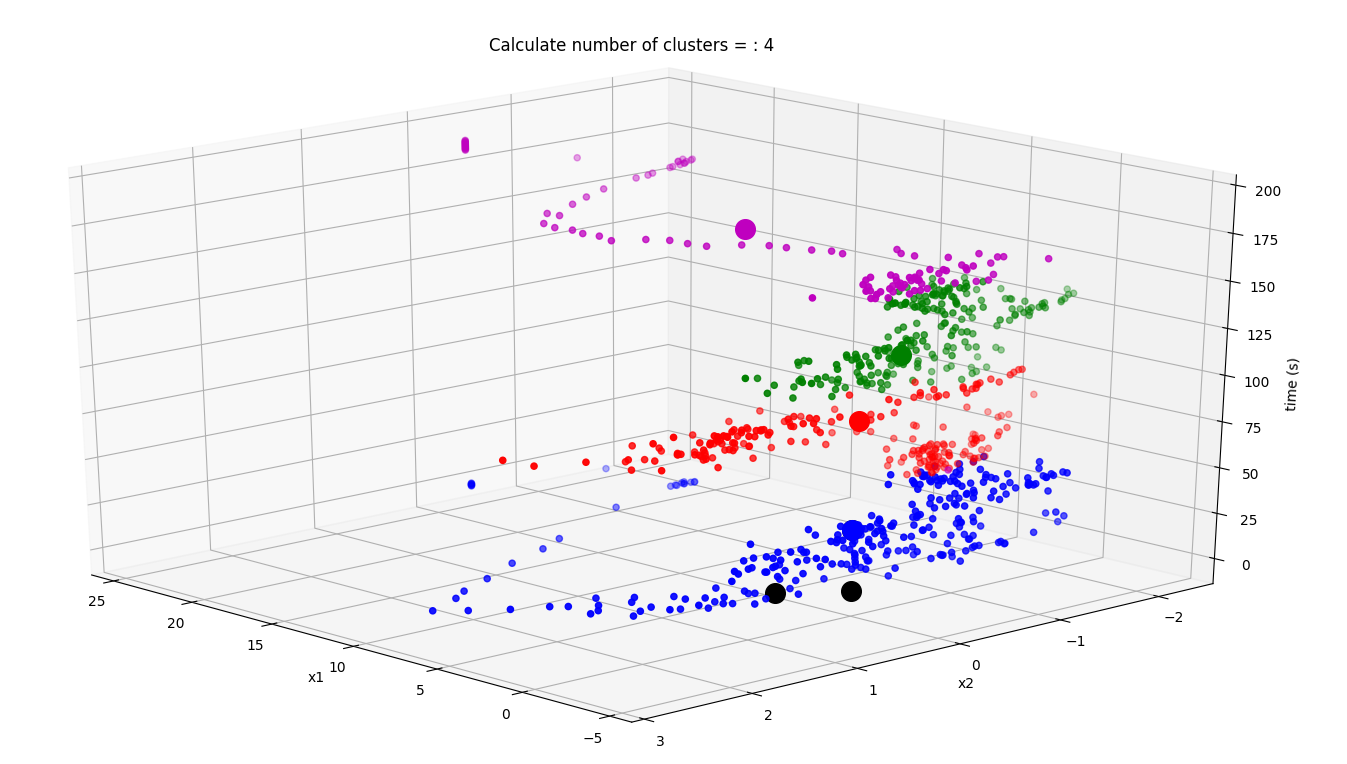
\includegraphics[width=1\linewidth]{clustering.png}
      \caption{Clustering results: the song is divdied into distinct sections. Each colour represents a different cluster, with the cluster centroid represented by the larger markers. x1 and x2 axes represent the reduce feature set, while the vertical axis is time.}
      \label{fig:clustering}
\end{figure}
\begin{figure}[H]
      \centering
      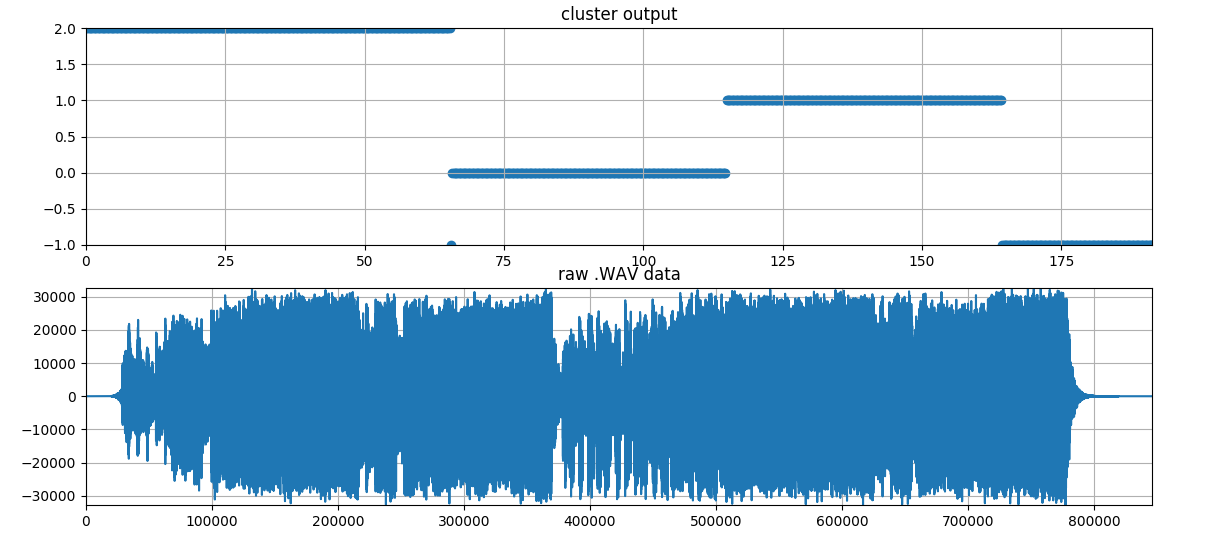
\includegraphics[width=1\linewidth]{cluster_output.png}
      \caption{An alternate view of the clustering results. The cluster number is plotted next to the raw song data.}
      \label{fig:cluster_output}
\end{figure}
\begin{figure}[H]
      \centering
      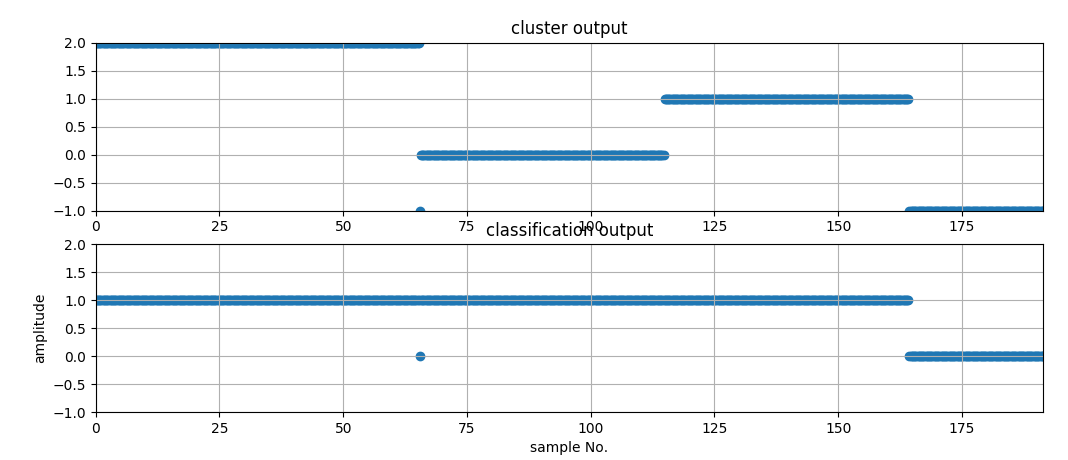
\includegraphics[width=1\linewidth]{classification.png}
      \caption{Classification results: Some songs performed better than others. In this case, the song sections are classified, but most of the song is labeled '1', which is a chorus section, with only the end of the song classified as a sparse section}
      \label{fig:classification}
\end{figure}

